% This is text associated with the open textbook "Open Electromagnetics"
% See immediately below for author, date
% This work is licensed under the Creative Commons Attribution-ShareAlike 4.0 International License. (CC BY-SA 4.0) 
% To view a copy of the license, visit http://creativecommons.org/licenses/by-sa/4.0/

%ORB TITLE Dispersion in Optical Fiber
%ORB AUTHOR 0        # S.W. Ellingson, Virginia Tech (ellingson@vt.edu)
%ORB DATE 20191124   # yyyymmdd
%ORB ABSTRACT 

\label{m0193_Dispersion_Optical_Fiber} % <-- Must match name of this file and module directory name.  Don't mess with this!
\index{optical fiber|(}

Light may follow a variety of paths through a fiber optic cable.  Each of the paths has a different length, leading to a phenomenon known as \emph{dispersion}.
\index{dispersion}
Dispersion distorts signals and limits the data rate of digital signals sent over fiber optic cable.
In this section, we analyze this dispersion and its effect on digital signals.

% multimode vs. single-mode

Figure~\ref{m0193_fFOModes} shows the variety of paths that light may take through a straight fiber optic cable.
%
\begin{figure}[b!] % <--- "[b]" for first figure in section *only*; delete for 2nd and subsequent figures
\begin{center}
\pdftooltip{{  % note double braces
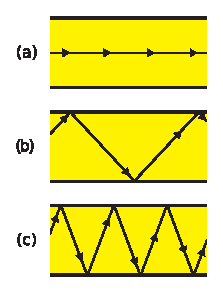
\includegraphics[width=2in]{modules/m0193_fFOModes.eps} 
% https://commons.wikimedia.org/wiki/File:Paths_of_Light_through_Optic_Cable.svg
}}{Diagram in three parts, a, b, and c. For a, wave travels horizontally. For b, wave travels at some angle with reflected wave creating wide triangles. For c, wave travels at maximum angle with reflected wave creating narrow triangle.}
\end{center}
\centerline{\scriptsize 
\copyright~\hyperref[m0193_fFOModes_Credit]{S.\ Lally} 
\href{https://creativecommons.org/licenses/by-sa/4.0/}{CC BY-SA 4.0} 
} % \centerline 
\caption{
\label{m0193_fFOModes}
Paths that light may take through a straight fiber optic cable: (a) Along axis, corresponding to minimum path length; (b) Intermediate between (a) and (c); (c) Maximum length, corresponding to threshold angle for total internal reflection.
}
\end{figure} 
%
The nominal path is shown in Figure~\ref{m0193_fFOModes}(a), which is parallel to the axis of the cable.  This path has the shortest associated propagation time.
The path with the longest associated propagation time is shown in Figure~\ref{m0193_fFOModes}(c).  In this case, light bounces within the fiber, each time approaching the core-clad interface at the critical angle for total internal reflection.  Any ray approaching at a greater angle is not completely reflected, and so would likely not survive to the end of the cable.
Figure~\ref{m0193_fFOModes}(b) represents the continuum of possibilities between the extreme cases of (a) and (c), with associated propagation times greater than that of case (a) but less than that of case (c).

Regardless of how light is inserted into the fiber, all possible paths depicted in Figure~\ref{m0193_fFOModes} are likely to exist.  This is because fiber is rarely installed in a straight line, but rather follows a multiply-curved path.  Each curve results in new angles of incidence upon the core-cladding boundary.  The existence of these paths leads to dispersion.  To see this, consider the input signal shown in Figure~\ref{m0193_fFiberDigIn}.
%
\begin{figure} % <--- "[b]" for first figure in section *only*; delete for 2nd and subsequent figures
\begin{center}
\pdftooltip{{  % note double braces
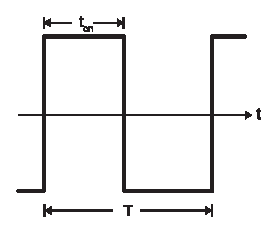
\includegraphics[width=2.5in]{modules/m0193_fFiberDigIn.eps} 
% https://commons.wikimedia.org/wiki/File:Digital_Signal_on_Fiber_Optic_Cable.svg
}}{A square wave shown with respect to time. The width of each square is small t subscript on and the period labeled capital t.}
\end{center}
\centerline{\scriptsize 
\copyright~\hyperref[m0193_fFiberDigIn_Credit]{S.\ Lally} 
\href{https://creativecommons.org/licenses/by-sa/4.0/}{CC BY-SA 4.0} 
} % \centerline 
\caption{
\label{m0193_fFiberDigIn}
A digital signal that might be applied to the input of a fiber optic cable.
}
\end{figure} 
%
This signal has period $T$, during which time a pulse of length $t_{on}<T$ may be present.
Let the \emph{minimum} propagation time through the fiber (as in Figure~\ref{m0193_fFOModes}(a)) be $\tau_{min}$.
Let the \emph{maximum} propagation time through the fiber (as in Figure~\ref{m0193_fFOModes}(c)) be $\tau_{max}$.
If $\tau_{max}-\tau_{min}\ll t_{on}$, we see little degradation in the signal output from the fiber.
Otherwise, we observe a ``smearing'' of pulses at the output of the fiber, as shown in Figure~\ref{m0193_fFiberDigOut}.
%
\begin{figure} % <--- "[b]" for first figure in section *only*; delete for 2nd and subsequent figures
\begin{center}
\pdftooltip{{  % note double braces
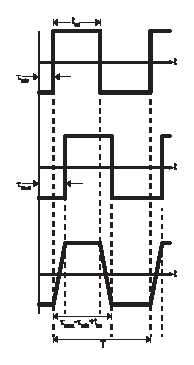
\includegraphics[width=2.5in]{modules/m0193_fFiberDigOut.eps} 
% https://commons.wikimedia.org/wiki/File:Dispersion_on_Signal_Output_from_Fiber_Optic_Cable.svg
}}{Three square waves are plotted over time small t. The first wave’s pulse starts at small tau subscript min, has pulse width small t subscript on, and period capital t. The second plot has a wave pulse that starts at small tau subscript max and has the same pulse width and period. The third plot shows the sum. The pulse begins at small tau subscript min reaches the max amplitude at small tau subscript max, and begins to fall at small t subscript on. The pulse width from rise to fall is tau subscript max minus tau subscript min plus t subscript on.}
\end{center}
\centerline{\scriptsize 
\copyright~\hyperref[m0193_fFiberDigOut_Credit]{S.\ Lally} 
\href{https://creativecommons.org/licenses/by-sa/4.0/}{CC BY-SA 4.0} 
} % \centerline 
\caption{
\label{m0193_fFiberDigOut}
The effect of dispersion on the signal output from the fiber optic cable:
\emph{Top:} Arriving waveform corresponding to minimum path length, 
\emph{Middle:} Arriving waveform corresponding to maximum path length, and
\emph{Bottom:} Sum of all arriving waveforms.
}
\end{figure} 

Any smearing may pose problems for whatever device is detecting pulses at the receiving end.
However, as $\tau_{max}-\tau_{min}$ becomes a larger fraction of $t_{on}$, we see that it becomes possible for adjacent pulses to overlap.
This presents a much more serious challenge in detecting individual pulses, so let us examine the overlap problem in greater detail.
To avoid overlap:
%
\begin{equation}
\tau_{max}-\tau_{min} + t_{on} < T
\end{equation}
%
Let us define the quantity $\tau \triangleq \tau_{max}-\tau_{min}$.
This is sometimes referred to as the \emph{delay spread}.\footnote{Full disclosure:  There are many ways to define ``delay spread,'' but this definition is not uncommon and is useful in the present analysis.}
\index{delay spread}
Thus, we obtain the following requirement for overlap-free transmission:
%
\begin{equation}
\tau < T - t_{on}
\end{equation}

Note that the delay spread imposes a minimum value on $T$, which in turn imposes a maximum value on the rate at which information can be transmitted on the cable.
So, we are motivated to calculate delay spread.
The minimum propagation time $t_{min}$ is simply the length $l$ of the cable divided by the phase velocity $v_p$ of the light within the core; 
i.e., $t_{min} = l/v_p$.  
Recall phase velocity is simply the speed of light in free space $c$ divided by $\sqrt{\epsilon_r}$ where $\epsilon_r$ is the relative permittivity of the core material.
Thus:
%
\begin{equation}
t_{min} = \frac{l}{v_p} = \frac{l}{c/\sqrt{\epsilon_r}} = \frac{l}{c/n_f} = \frac{l n_f}{c}
\end{equation}
%
The maximum propagation time $t_{max}$ is different because the maximum path length is different. 
Specifically, the maximum path length is not $l$, but rather $l/\cos\theta_2$ where $\theta_2$ is the angle between the axis and the direction of travel as light crosses the axis.
So, for example, $\theta_2=0$ for $t_{min}$ since light in that case travels along the axis.
The value of $\theta_2$ for $t_{max}$ is determined by the threshold angle for total internal reflection.
This was determined in Section~\ref{m0192_Acceptance_Angle} to be given by:
%
\begin{equation}
\cos\theta_2 = \frac{n_c}{n_f} ~~~~~~\mbox{(threshold value)}
\end{equation}
%
so we obtain the following relationship:
%
\begin{equation}
t_{max} = \frac{l/\cos\theta_2}{v_p} = \frac{l n_f/n_c}{c/n_f} = \frac{l n_f^2}{c n_c}
\end{equation}
%
and subsequently we find:
%
\begin{equation}
\boxed{
\tau = l \frac{n_f}{c} \left( \frac{n_f}{n_c} - 1 \right)
}
\label{m0193_eDS}
\end{equation}
%
Note that $\tau$ increases linearly with $l$.
Therefore, the rate at which pulses can be sent without overlap decreases linearly with increasing length.
In practical applications, this means that the maximum supportable data rate decreases as the length of the cable increases.
This is true independently of media loss within the cable (which we have not yet even considered!).
Rather, this is a fundamental limitation resulting from dispersion.

%%%%%%%%%%%%%%%%%%%%%%%%%%%%%%%%%%%%%%%%%%%%%%%
%ORB EXAMPLE
~\\ \begin{example} 
\begin{mdframed}[backgroundcolor=brown!20,linecolor=brown!20]\raggedright
Maximum supportable data rate in multimode fiber optic cable.
\\~\\  
A multimode fiber optic cable of length 1~m is used to transmit data using the scheme shown in Figure~\ref{m0193_fFiberDigIn}, with $t_{on}=T/2$.
Values of $n_f$ and $n_c$ for this fiber are 1.52 and 1.49, respectively.
What is the maximum supportable data rate?

{\bf Solution}. 
Using Equation~\ref{m0193_eDS}, we find the delay spread $\tau\cong 102$~ps.
To avoid overlap, $T>2\tau$; therefore, $T$ greater than about 204~ps is required.
The modulation scheme allows one bit per period, so the maximum data rate is $1/T\cong 4.9\times 10^9$~bits per second; i.e., $\cong$ \underline{4.9~Gb/s}.
\end{mdframed}
% note figures will need to go between "\end{mdframed}" and "\end{example}"
\end{example}
%%%%%%%%%%%%%%%%%%%%%%%%%%%%%%%%%%%%%%%%%%%%%%%

The finding of 4.9~Gb/s may seem like a pretty high data rate; however, consider what happens if the length increases to 1~km.  It is apparent from Equation~\ref{m0193_eDS} that the delay spread will increase by a factor of 1000, so the maximum supportable data rate decreases by a factor of 1000 to a scant 4.9~Mb/s.
Again, this is independent of any media loss within the fiber.
To restore the higher data rate over this longer path, the dispersion must be reduced.
One way to do this is to divide the link into smaller links separated by repeaters which can receive the dispersed signal, demodulate it, regenerate the original signal, and transmit the restored signal to the next repeater.
Alternatively, one may employ ``single mode'' fiber, which has intrinsically less dispersion than the multimode fiber presumed in our analysis.

%%%%%%%%%%%%%%%%%%%%%

{\bf Additional Reading:}
\begin{itemize}
\item ``\href{https://en.wikipedia.org/wiki/Optical_fiber}{Optical fiber}'' on Wikipedia.
\end{itemize}

\index{optical fiber|)}


